\section{LA-CDIP Dataset}
\label{sec:dataset}

The proposed dataset is composed of 4993 documents, divided in 144 different classes. Each class has at least two documents, the biggest class has 497 documents, and the median size of the classes is 13, exposing an extra challenge on dealing with a unbalanced dataset. \refFig{fig:histplot} shows the class distribution.

\begin{figure}[htbp]
\centering
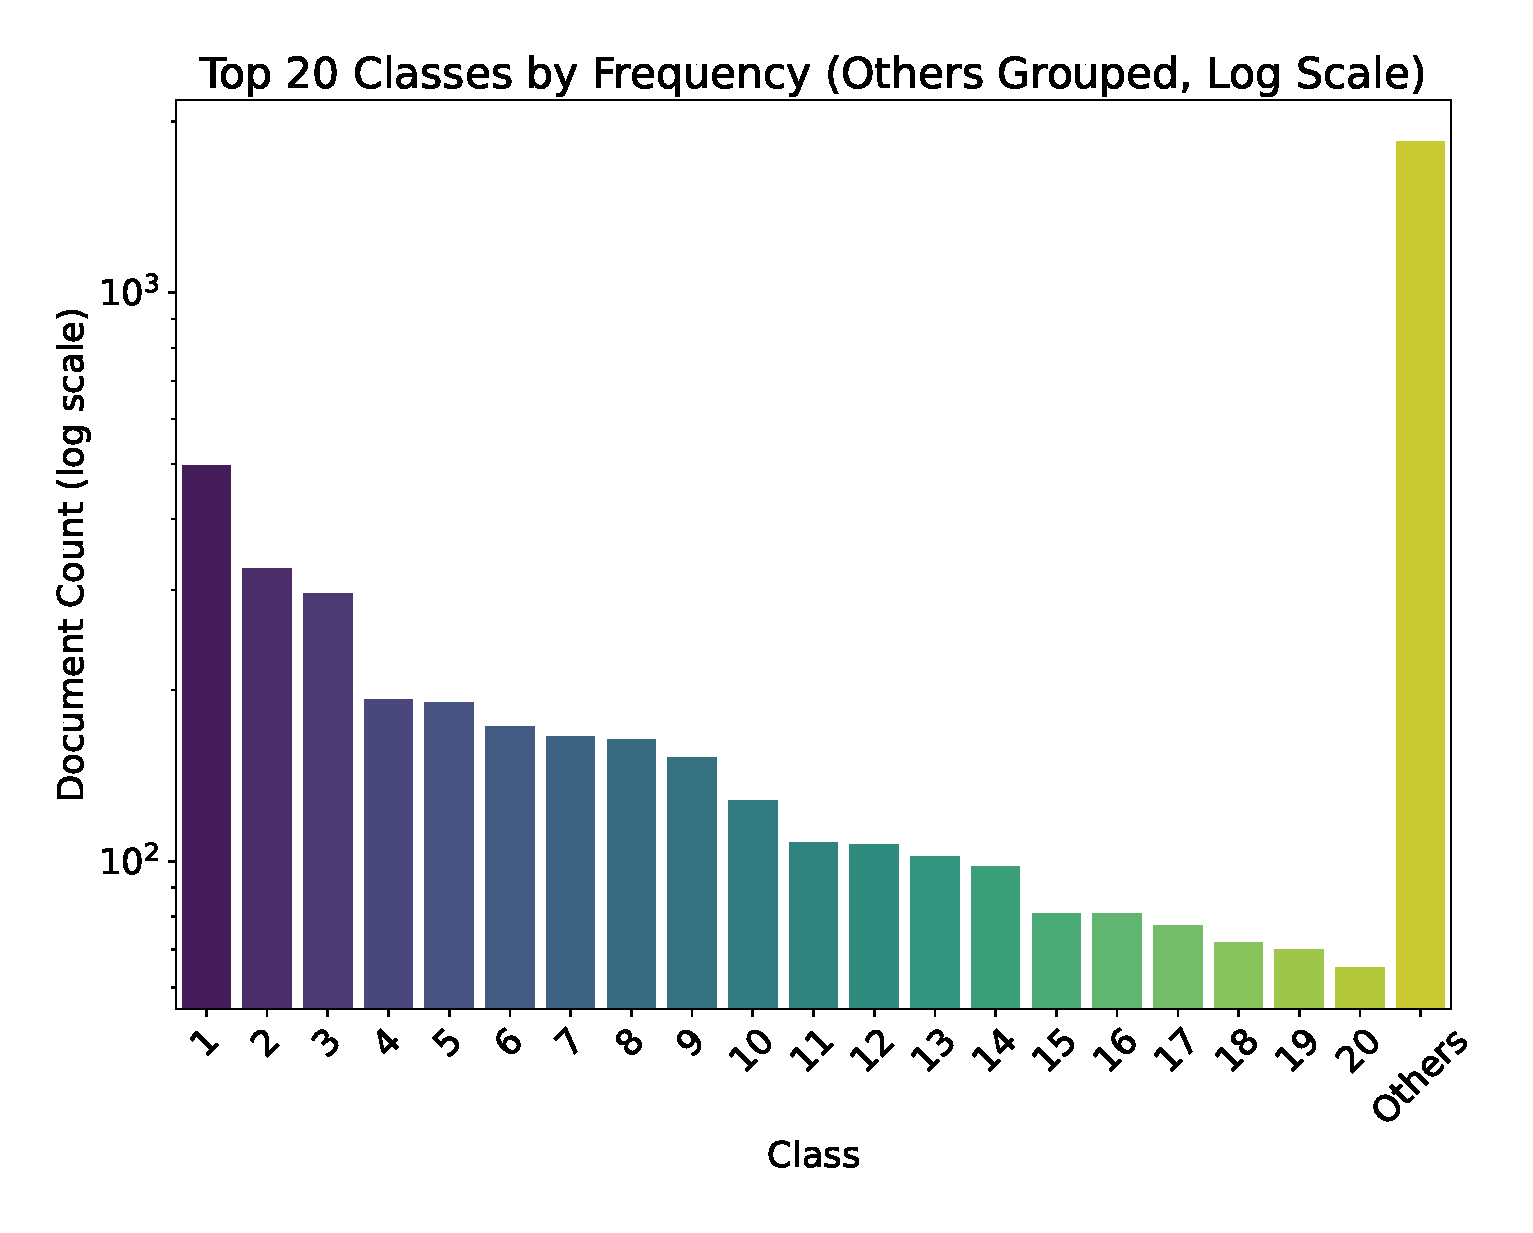
\includegraphics[width=.8\textwidth]{images/hist2.eps}
\caption{Histogram showing the top 20 classes by their frequency. The other 124 classes are grouped in the ``others'' column. Note that the plot is in log scale.}
\label{fig:histplot}
\end{figure}  

To maintain train-test data consistency, the data is split following the \gls{ZSL} and \gls{GZSL} protocols proposed by Xian et al \cite{gzsl}. Each protocol is a different method to split train and test data: \gls{ZSL} is the complete separation of train and test classes - no overlap between the splits; while the \gls{GZSL} follows a more realistic scenario by partially overlapping train and test classes, having half the test or validation set be of seen classes, and half of unseen classes. In both scenarios, the data is split into train and test data, and the train data is further divided by a 5-fold cross-validation \cite{kfoldcv}.

The data for the test scenario and the data for each split are chosen randomly, and the same for every experiment. The test scenario is picked as a sixth split for the cross-validation, so it follows the same rules for the other 5 splits. For the \gls{ZSL} scenario, a sixth of the classes are randomly chosen for each split, with no overlapping. Naturally, this scenario creates splits with variable sizes, as the classes themselves have variable sizes. For the \gls{GZSL} scenario, half the classes in the whole dataset are chosen as classes that do not overlap between splits, and other half are diluted between the splits. While constructing a split, first, the non overlapping classes are chosen for the split, then the remaining slots are filled with the overlapped classes, achieving splits with a constant size for this scenario.

This dataset can be used for a traditional visual classification problem, but since the problem is tackled with metric learning, additional considerations must be taken into account. While using a Siamese network, running inference on a single point of data returns no information, as the architecture requires some sort of comparison between different data points. Randomly selecting pairs every test can fluctuate the results, therefore, to maintain the test consistency, a test protocol is used that assures the same pairs are tested every time. For every document in the set, two other documents are chosen: one that shares the same class, and one that does not. This document is chosen randomly by its class, therefore, every class has the same probability of being picked. A protocol exists for the test set and for every cross-validation split.


\section{Evaluation Criteria}
\label{sec:evaluation}

Since a metric learning model yields a distance between two data points (in this case, two documents), a threshold needs to be defined to declare whether the two data points belong to the same class or not, to calculate how accurate the model is. For this, \gls{EER} is used as the metric for the experiments~\cite{EER}. \gls{EER} is  the point at which the \gls{FAR} and \gls{FRR} are equal. The \gls{EER} is calculated by setting the \gls{FAR} equal to the \gls{FRR} and finding the corresponding threshold at this point~\cite{EER2}. In other words, the \gls{EER} is the value of error rate when the threshold value $\tau_{EER}$ gives 
\begin{equation}
    FAR(\tau_{EER}) = FRR(\tau_{EER}),
\end{equation}
where
\begin{equation} \label{far}
    FAR(\tau) = \frac{\text{Number of false acceptances at threshold~} \tau}{\text{Total number of negative samples}}
\end{equation}
is the probability that a negative sample is incorrectly classified as positive~\cite{EER3}. On the other hand,
\begin{equation} \label{frr}
    FRR(\tau) = \frac{\text{Number of false rejections at threshold~} \tau}{\text{Total number of positive samples}}
\end{equation}
is the probability that a positive sample (e.g., a genuine user) is incorrectly classified as negative.

Ten models are trained for each chosen backbone (see \refCap{sec:method_modeling}): a 5-fold cross-validation for each of the 2 scenarios, \gls{ZSL} and \gls{GZSL}. As shown in Section \ref{sec:method_dataset}, each split follows a fixed validation protocol to ensure consistency. The trained models from each split are also evaluated on the independent test set, to compare them with the \gls{LLM}s. The mean \gls{EER} is reported for every cross-validation scenario, as well as the mean \gls{EER} on the independent test set.

\section{LLMs}

For the \glspl{LLM} analysis, the chosen models are LLaVA 3.2 Vision, InternVL 2.5, Qwen2.5-VL, GPT-4o (2024-11-20), and GPT-4o-mini (2024-07-18). They were chosen given their performance in document understanding benchmarks~\cite{bai2025qwen2,meta2024llama3.2}, which  demonstrated capabilities in tasks involving visual-text reasoning, OCR, and layout-based document analysis. These models were evaluated in a zero-shot manner, without any fine-tuning or additional training.

\section{Partial Results}
\label{sec:results}

The results of the research are presented in this chatper. This chapters's discussions revolves around Table \ref{tab:res}, where the results of every trained model are presented. The table shows the mean EER value of the cross-validation in both scenarios, as well as the mean performance of each fold on the independent test set. While the \gls{ZSL} and the \gls{GZSL} scenarios are very influential on the visual models performance, this difference is not relevant on the \gls{LLM} test, as they have not been fine-tuned for the task. While they may have been originally trained with some documents of the RVL-CDIP database, both scenarios are effectively \gls{ZSL}. The \refCap{sec:visual_models} discusses the results of the trained visual models and compare the effects of different backbones in the result. \refCap{sec:llm_result}, compares the results returned by the multimodal \glspl{LLM} chosen for this work. Finally, \refCap{sec:comparison_result}, compares both approaches.

\begin{table}[ht]
\caption{Comparative performance between different visual backbones and Large Language Models. Following the columns: the architecture name, the architecture edition, if exists, cross-validation over the \gls{ZSL} scenario, cross-validation over the \gls{GZSL} scenario, test performance on the \gls{ZSL} scenario, and test performance over the \gls{GZSL} scenario. Every value is a mean EER (\%) value over the \gls{CV} folds.}
\label{tab:res}
\centering
\setlength{\tabcolsep}{6pt}
\begin{tabular}{lclcccc}
\toprule
Architecture                            & Edition & Params & \gls{ZSL}    & \gls{GZSL}    & Test \gls{ZSL} & Test \gls{GZSL} \\
\midrule
AlexNet                                 &         &  57M   & 8.92   & 5.45    & 17.33    & 6.31      \\ \midrule
\multirow{4}{*}{VGG}                    & 11      &  129M  & 7.47   & 5.01    & 14.24    & 3.95      \\
                                        & 13      &  129M  & 7.03   & 4.79    & 9.30     & 3.95      \\
                                        & 16      &  134M  & 8.29   & 5.23    & 14.74    & 4.82      \\
                                        & 19      &  139M  & 7.30   & 4.57    & 17.08    & 3.90      \\ \midrule
\multirow{5}{*}{ResNet}                 & 18      &  11M   & 5.03   & 1.54    & 4.98     & 1.51      \\
                                        & 34      &  21M   & 4.32   & 2.10    & 4.13     & 1.53      \\
                                        & 50      &  23M   & 6.90   & 3.39    & 10.34    & 2.21      \\
                                        & 101     &  42M   & 8.20   & 2.72    & 11.31    & 1.98      \\
                                        & 152     &  58M   & 9.44   & 3.38    & 12.70    & 2.39      \\ \midrule
\multirow{2}{*}{MobileNetV3}            & Small   &  1M    & 7.98   & 5.06    & 12.74    & 5.26      \\
                                        & Large   &  4M    & 8.16   & 4.27    & 8.45     & 4.43      \\ \midrule
\multirow{4}{*}{EfficientNet}           & 0       &  4M    & 4.41   & 2.27    & 6.02     & 0.95      \\
                                        & 1       &  6M    & 3.93   & 3.54    & 8.88     & 2.70      \\
                                        & 2       &  7M    & 5.73   & 2.61    & 7.29     & 2.14      \\
                                        & 3       &  10M   & 5.65   & 3.64    & 7.37     & 2.34      \\ \midrule
\multirow{2}{*}{\gls{ViT}}              & Base    &  87M   & 12.43  & 7.97    & 19.72    & 5.19      \\
                                        & Large   &  305M  & 13.16  & 7.57    & 19.88    & 5.26      \\ \midrule
Llama                                &  3.2     &     11B   & --     & --      & 13.95    & 21.90     \\
InternVL                             & 2.5      &   8B     & --     & --      & 8.58     & 10.40     \\
Qwen-VL                              & 2.5       &   7B     & --     & --      & 6.61     & 4.20      \\
GPT 4o mini                                 & 2024-07-18    &   *     & --     & --      & 4.70     & 4.07      \\
GPT 4o                                  & 2024-11-20      &    *    & --     & --      & 2.75     & 1.33      \\ \bottomrule

\end{tabular}
\smallskip
\parbox[t]{\textwidth}{\footnotesize
    * The parameter count of GPT-4o has not been publicly disclosed.}
\end{table}

\subsection{Visual Models}
\label{sec:visual_models}

Among visual models, smaller and more cost-efficient architectures outperformed larger ones. This trend is evident in different ResNet variants: ResNet-18 and ResNet-34 showed strong performance, while larger versions (ResNet-50, ResNet-101, and ResNet-152) performed progressively worse. Additionally, the \gls{ViT}, despite excelling on datasets like ImageNet \cite{imagenet}, was the worst-performing model in this task. Figure \ref{fig:tsne} shows that, while none of the class separations are perfect, ResNet-18 and EfficientNet-b0 have a better inter-class separation, if compared against ViT-b and ViT-l. These larger models overfitted to the training data, with some reaching 0\% train error in certain epochs while maintaining a high validation error. The most likely cause of this behavior is the dataset size—LA-CDIP contains only 4,993 documents, with approximately two-thirds used for training in each fold. However, techniques such as tuple mining and data augmentation could help mitigate this effect by increasing the diversity of training samples and improving feature learning. The overall best models are the ResNet-34, and EfficientNet-0 and 1. They offer a balance in size, achieving a good generalization of the problem while also learning the intricacies the task demands.

\begin{figure}[htbp]
    \centering
    \begin{minipage}{0.4\linewidth}
        \centering
        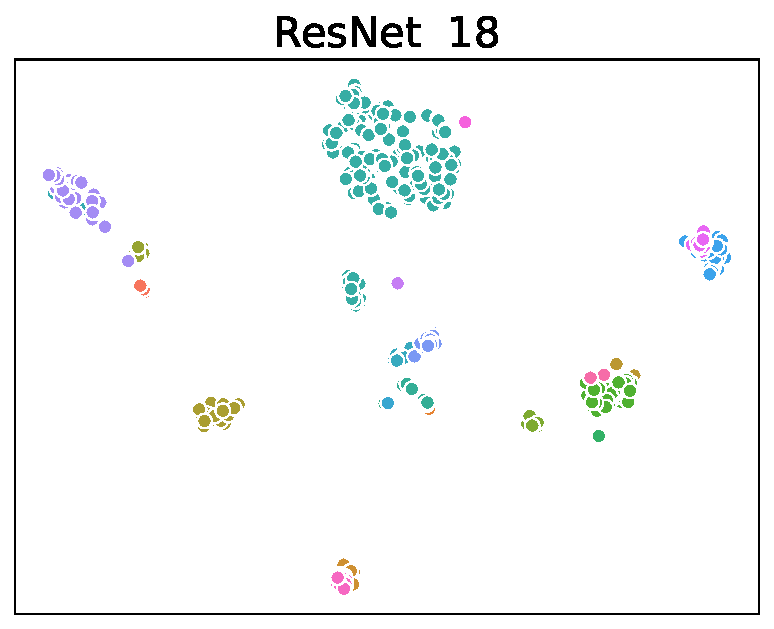
\includegraphics[width=\linewidth]{images/ResNet.csv_18_0.pdf}
        % \caption{Similar Comparison}
    \end{minipage}
    \begin{minipage}{0.4\linewidth}
        \centering
        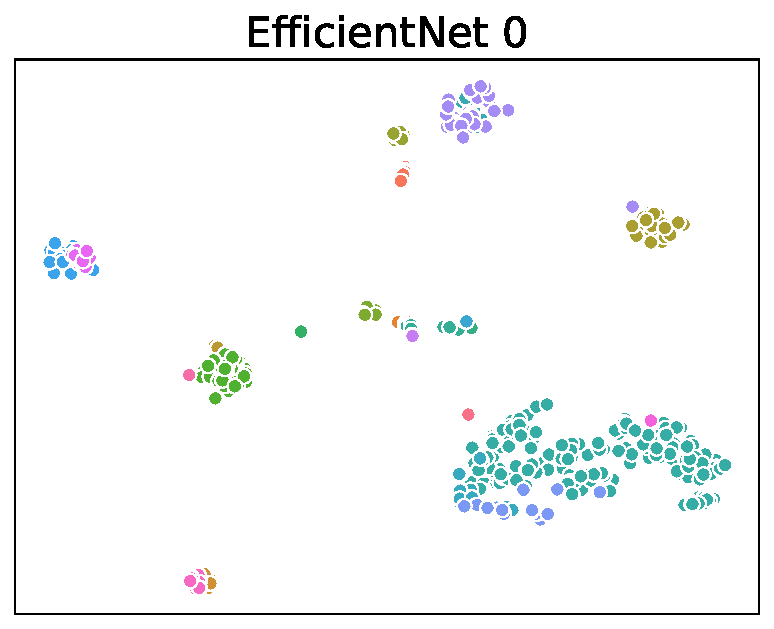
\includegraphics[width=\linewidth]{images/EfficientNet.csv_0_0.pdf}
        % \caption{Different Comparison}
    \end{minipage}
    \begin{minipage}{0.4\linewidth}
        \centering
        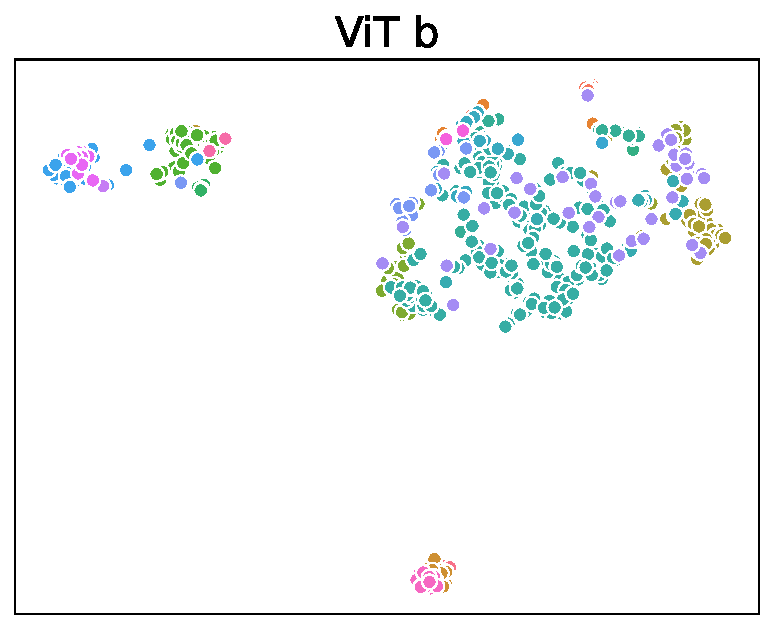
\includegraphics[width=\linewidth]{images/ViT.csv_b_0.pdf}
        % \caption{Different Comparison}
    \end{minipage}
    \begin{minipage}{0.4\linewidth}
        \centering
        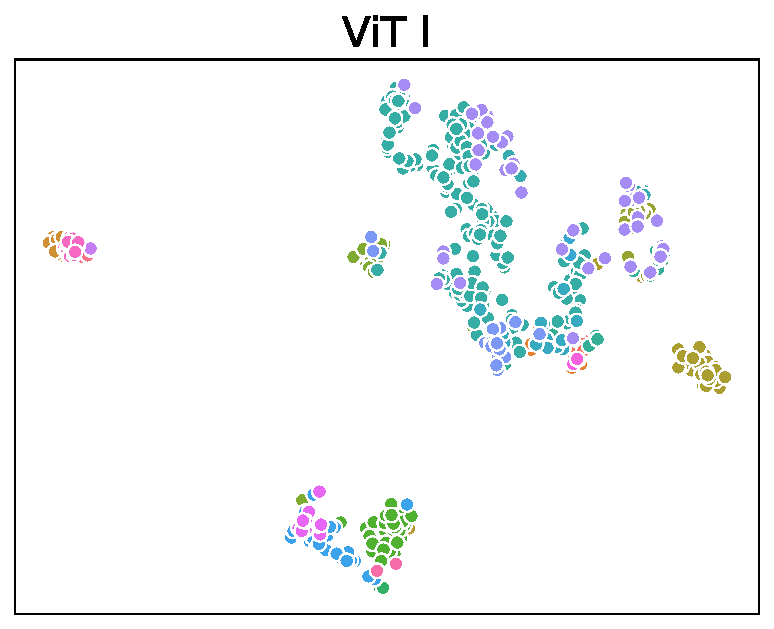
\includegraphics[width=\linewidth]{images/ViT.csv_l_0.pdf}
        % \caption{Different Comparison}
    \end{minipage}
    \caption{TSNE visualization of the Test ZSL scenario. These models have been trained on the same cross-validation fold.\label{fig:tsne}}
\end{figure}

Comparing the \gls{ZSL} and the \gls{GZSL} results, the \gls{GZSL} consistently gives better results. This is expected, since half of the validation set on each fold is composed of classes seen in training. The biggest discrepancies between the two modalities can be seen in the largest models, where the overfitting damage is mitigated by the easier scenario. Even so, the best performance on the \gls{GZSL} scenario is usually connected with a good performance on the \gls{ZSL} scenario.

In the test scenarios, the reported values represent the mean performance across all folds, evaluated on the same set. Since this is a Zero-shot data split, there is inherently a high variance over the different splits, since they test on entirely different patterns each fold. By chance, the \gls{ZSL} test split is more challenging than average, resulting in higher error rates for most models relative to the mean cross-validation error rate. The test \gls{GZSL} scenario follows the opposite reasoning.

\subsection{Large Language Models}
\label{sec:llm_result}

All models were tested under similar conditions, however, further performance improvements could be achieved through refined prompt engineering. Therefore, the results presented should not be considered as definitive comparisons of the models capabilities but rather a baseline for assessing the viability of the proposed method. Despite these limitations, \gls{LLM} results align with existing benchmarks for document understanding tasks for these models. 

As shown in Table~\ref{tab:res}, GPT-4o exhibited the best overall performance, achieving the lowest error rates in both the \gls{ZSL} and \gls{GZSL} scenarios. The GPT-4o-mini variant performed similarly but showed slightly lower accuracy, reflecting its trade-off between efficiency and capability.

Additionally, Llama 3.2 Vision faced challenges in handling multiple document inputs, requiring images to be combined into a single input before processing. This limitation impacted its ability to directly compare layouts across distinct documents, differentiating its approach from the other evaluated models.

InternVL 2.5 and Qwen2.5-VL emerged as open-source alternatives for  \gls{ZSL} \gls{VDM}. Notably, the QwenVL 7B model reached performance levels close to those of GPT-4o mini, further highlighting the efficiency of these compact architectures.

Since the \glspl{LLM} have not been fine-tuned with the training data, the only difference between the \gls{ZSL} and \gls{GZSL} scenarios is the number of classes to compare: \gls{ZSL} has exactly $\frac{1}{6}$ of the classes and \gls{GZSL} can have every class, making \gls{GZSL} a more diverse test. Surprisingly, the two models performed with different trends between both scenarios: InternVL was better at the \gls{ZSL} split, and GPT better at the \gls{GZSL} split.

\subsection{Comparison}
\label{sec:comparison_result}

Given that \gls{GZSL} is an advantageous scenario for vision models—since they have been trained on half of the classes—while \glspl{LLM} have not been fine-tuned for this task, both settings effectively serve as pure zero-shot evaluations. Therefore, the comparison was conducted in the \gls{ZSL} scenario.

When compared to most \glspl{LLM}, \gls{LA-ZSL} enabled visual models to handle \gls{ZSL} \gls{VDM} while maintaining a significantly lower parameter count. This relationship between performance and model efficiency is illustrated in Figure~\ref{fig:performance}.

\begin{figure}[htbp]
\centering
%\isPreprints{\centering}{} % Only used for preprints
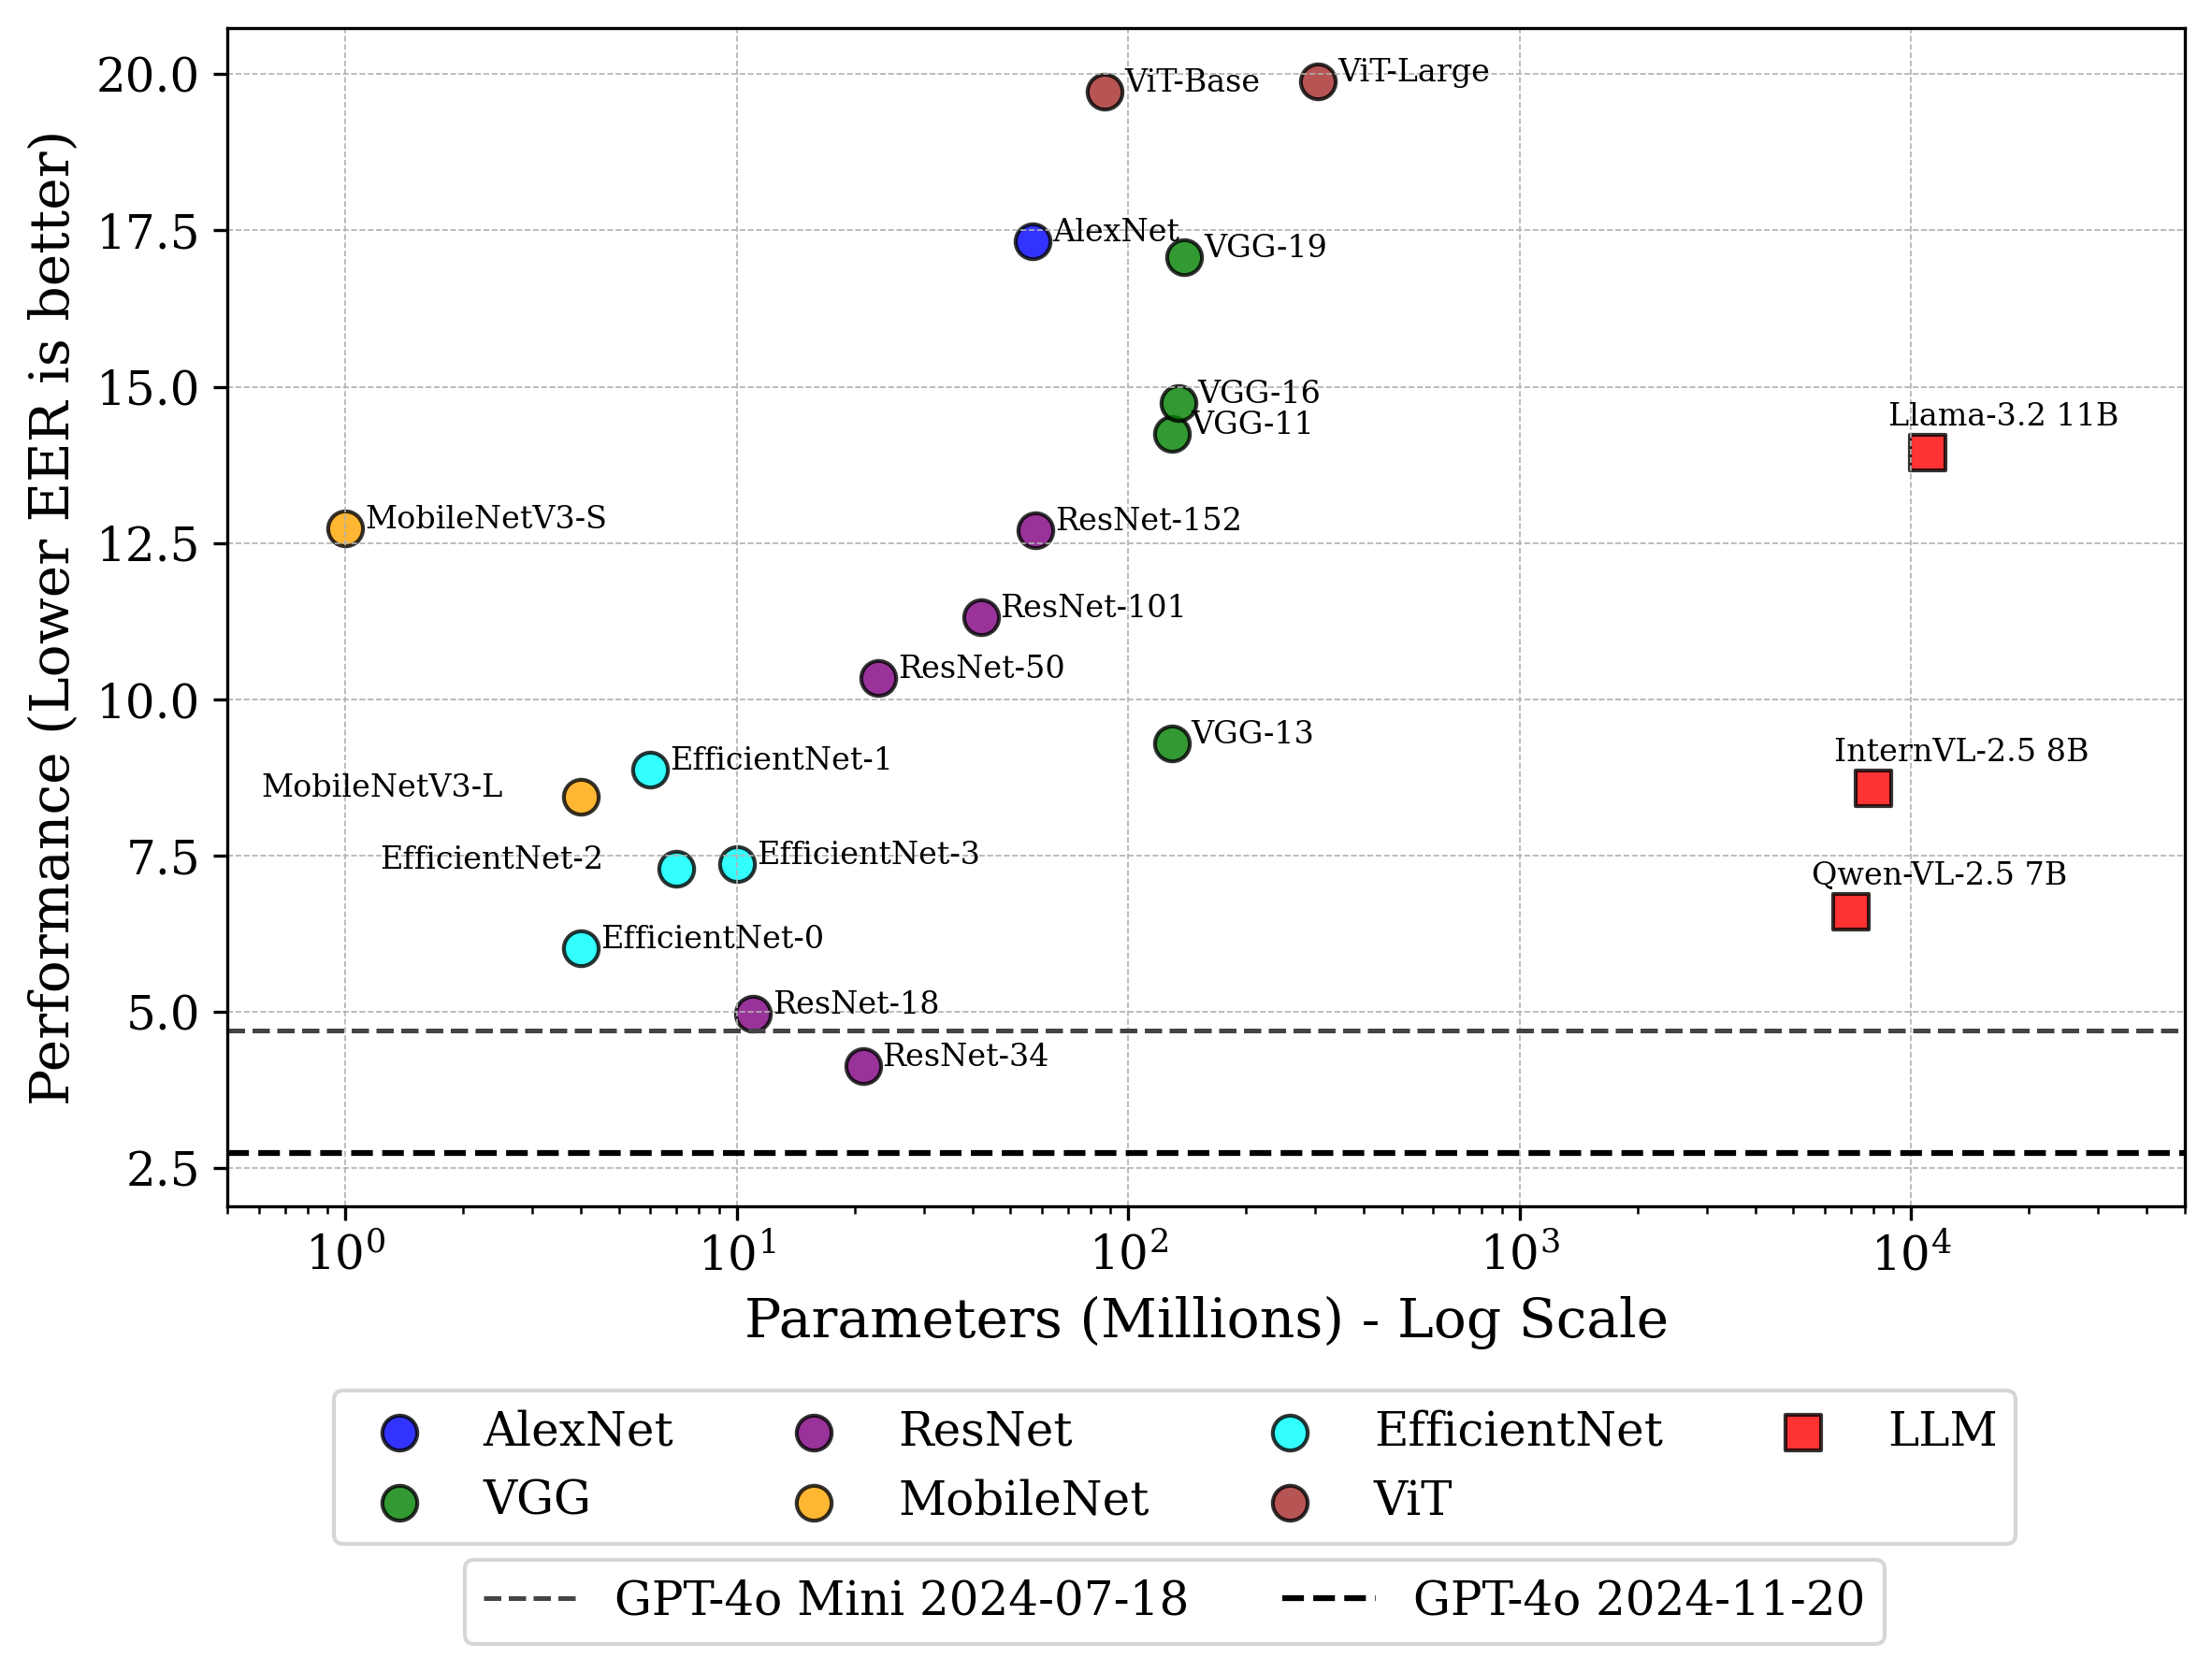
\includegraphics[width=1\linewidth]{images/performance_vs_parameters.png}
\caption{Performance vs Parameters (\acrlong{ZSL} scenario)\label{fig:performance}. The lines reprensent GPT-4o and GPT-4o Mini error rates, as their parameter count were not publicly disclosed.}
\end{figure}  

The results highlight a trade-off between model complexity and effectiveness. Smaller visual backbones, such as ResNet-18 and EfficientNet-0, achieve competitive performance while using significantly fewer parameters than large multimodal models. Notably, ResNet-18 and ResNet-34 exhibit lower error rates than several larger architectures, reinforcing the efficiency of lightweight vision models in document matching tasks.
